\documentclass[11pt, a4paper]{article}

\usepackage{graphicx}
\usepackage[a4paper,top=3cm,bottom=2cm,left=2cm,right=2cm,marginparwidth=1.75cm]{geometry}
\usepackage[english]{babel}
\usepackage[utf8x]{inputenc}
\usepackage{subfig}
\usepackage{float}
\usepackage{amsmath}
\usepackage{amssymb}
\usepackage{mhchem}
\usepackage{hyperref}
\usepackage{tikz}
\usepackage{cancel}

\graphicspath{ {./images} }
\newcommand*{\qed}{\hfill\ensuremath{\quad\square}}%
\newcommand*{\rad}{\ensuremath{\,\text{rad}}}
\newcommand*{\R}{\ensuremath{\mathbb{R}}}
\newcommand*{\C}{\ensuremath{\mathbb{C}}}
\renewcommand*{\Re}{\operatorname{Re}}
\renewcommand*{\Im}{\operatorname{Im}}
\renewcommand*{\epsilon}{\varepsilon}
\renewcommand*{\phi}{\varphi}

\makeatletter
\renewcommand*\env@matrix[1][*\c@MaxMatrixCols c]{%
  \hskip -\arraycolsep
  \let\@ifnextchar\new@ifnextchar
  \array{#1}}
\makeatother

\newtheorem{theorem}{Theorem}

%------------------------------------------------
%Templates for images and figures
% \begin{figure}[h]
%   \centering
%   \subfloat[caption 1]{{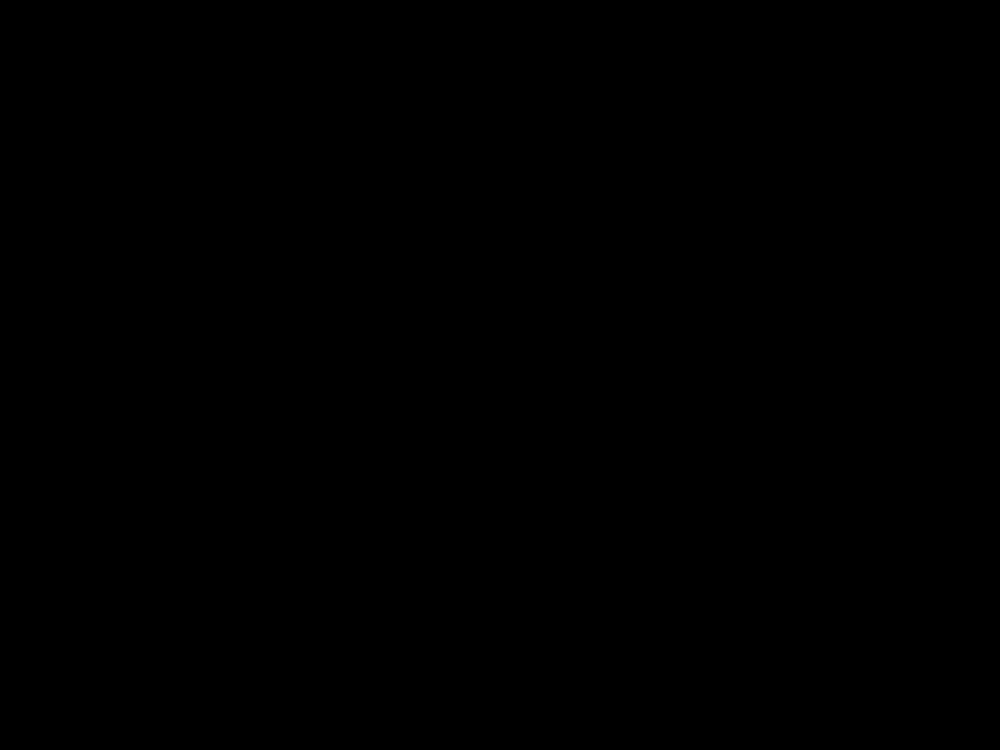
\includegraphics[width=30mm]{images/placeholder.png}}}%
%   \qquad
%   \subfloat[caption 2]{{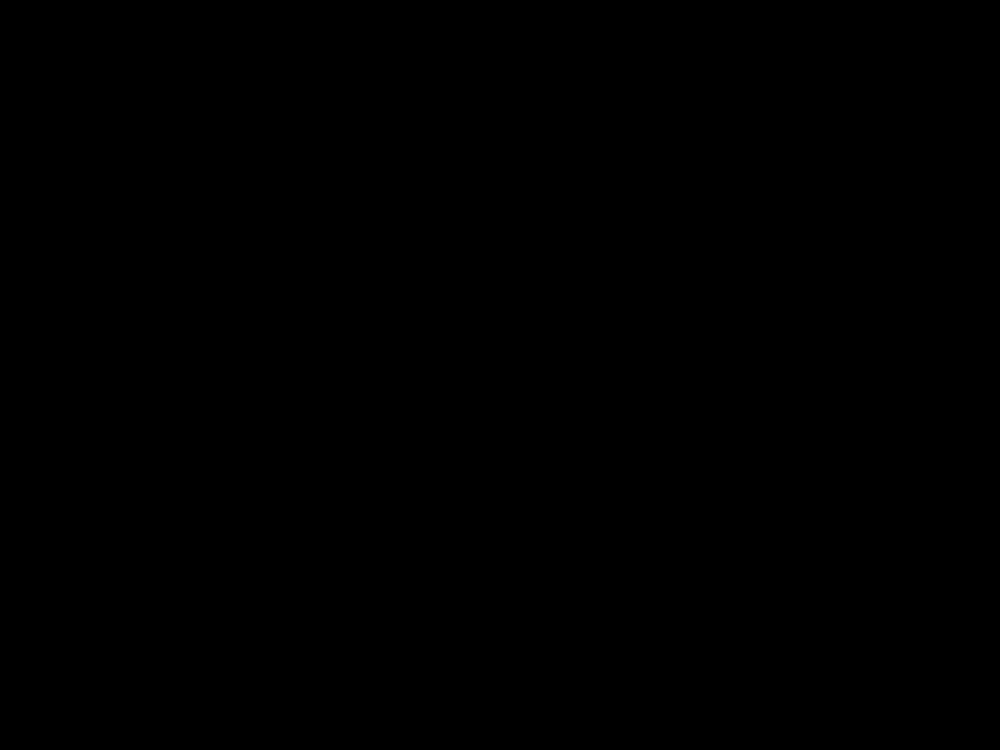
\includegraphics[width=30mm]{images/placeholder.png}}}%
%   \caption{Description}
% \end{figure}

% \begin{figure}[h]
%   \centerline{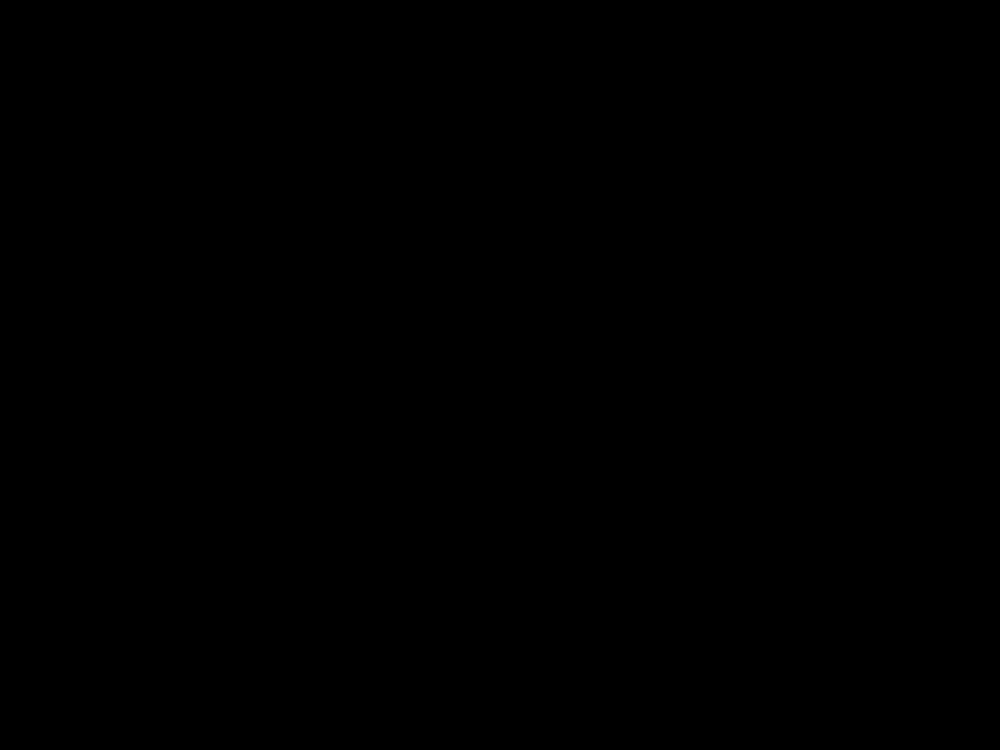
\includegraphics[width=50mm]{images/placeholder.png}}
%   \caption{Description}
% \end{figure}

%Template for a simple table 
%\begin{table}[h]
%   \caption{Description} %title of the table
%   \centering % centering table
%   \begin{tabular}{l rr} % creating three columns
%     \hline\hline %inserting double-line
%     & & \\ [0.5ex] % Insert half line vertical spacing
%     \hline % inserts single-line
%     & & \\ 
%     & & \\
%     & & \\
%     & & \\
%   \hline % inserts single-line
%   \end{tabular}
%   \label{tab:hresult}
% \end{table}
%-----------------------------------------------

\begin{document}
\setcounter{section}{7}
\setcounter{equation}{0}

\section{Linear Algebra 2 Lecture 8: Systems of differential equation*s (19/05/2020)}


\subsection{Recap on Differential equations}
Recall from analysis 1 \& 2 (WBMT1050) linear first and second order ordinary differential equations.\\
\underline{1st order linear ODE:}
\begin{equation*}
  y' = ay
\end{equation*}
Which has the general solution:
\begin{equation*}
  y(t) = ce^{at},\; c \in \R
\end{equation*}\\
\underline{homogeneous 2nd order linear ODE:}
\begin{equation*}
  y'' + ay' + by = 0
\end{equation*}
We solve this with black-mathemagics and geussing that the solution is of the form $y=e^{rt}$. Thus:
\begin{equation*}
  \begin{cases}
    y = e^{rt}\\
    y' = re^{rt}\\
    y'' = r^2e^{rt}
  \end{cases}
\end{equation*}
Subsituting this back into our original differential equation then gives:
\begin{equation*}
  r^2e^{rt} + are^{rt} + be^{rt} = 0
\end{equation*}
Since $e^{rt}\neq 0$ for any value of $r$ or $t$ we can divide it out leaving us with the characteristic equation:
\begin{equation*}
  r^2 + ar + b = 0
\end{equation*} 
Which has the following solution for $r_{1,2}$:
\begin{equation*}
  r_{1,2} = \frac{-a \pm \sqrt{a^2 - 4b}}{2}
\end{equation*}
The general solution for the differential equation then becomes:
\begin{equation*}
  y(t) = c_1e^{r_1t} + c_2e^{r_2t}, \; r_1, r_2 \in \R
\end{equation*}


\subsection{Linear systems of differential equations represented as vectors}
We can write a linear system of first order differential equations as follows:
\begin{equation*}
  \vec{x}'(t) = A\vec{x}
\end{equation*}
Where $A$ is some $n \times n$ matrix. Note the similarity to differential equations of the form $y' = ay$. We can again use black-mathemagics and geuss the solution takes the form $\vec{x}(t) = \vec{v}e^{\lambda t}$ where $\lambda$ is some eigenvalue of $A$ and $v$ a corresponding eigenvector. This leaves us with the following:
\begin{gather*}
  \vec{x}(t) = \vec{v}e^{\lambda t} \Rightarrow
  \begin{cases}
    x_1 = v_1 e^{\lambda t}\\
    x_2 = v_2 e^{\lambda t}
  \end{cases}\\
  \vec{x}'(t) = \lambda\vec{v}e^{\lambda t} \Rightarrow
  \begin{cases}
    x'_1 = v_1 \lambda e^{\lambda t}\\
    x'_2 = v_2 \lambda e^{\lambda t}
  \end{cases}\\
\end{gather*}
Subsituting this back into the original system leaves us with:
\begin{equation*}
  \lambda \vec{v} e^{\lambda t} = A\vec{v}e^{\lambda t}
\end{equation*}
Since $e^{\lambda t}$ will always be some non-zero scalar value we can divide it out, leaving us with:
\begin{equation*}
  \lambda \vec{v} = A\vec{v}  
\end{equation*}
This proves that the original guess that the solution takes the form $e^{\lambda t}$ is indeed valid. From this we can conclude that functions of the form $\vec{x}'(t) = A\vec{x}(t)$ has solutions of the form $\vec{v}e^{\lambda t}$. \\
For example: let $A$ be some $2 \times 2$ matrix with the eigenvalues $\lambda_1$ and $\lambda_2$. These eigenvalues have the corresponding eigenvectors $\vec{v}_1$ and $\vec{v}_2$. The solutions to the linear system of differential equations given by $\vec{x}'(t) = A\vec{x}(t)$ then becomes:
\begin{equation*}
  \vec{x}_1(t) = \vec{v}_1e^{\lambda_1 t},\; \vec{x}_2(t) = \vec{v}_2e^{\lambda_2 t}
\end{equation*}
Where $\vec{x}_1$ and $\vec{x}_2$ are generally referred to as eigenfunctions. it can be proven\footnote{but I'm not fucking going to} that any linear combination of these eigenfunctions is also a solution. Thus we can express the general solution to $\vec{x}'(t) = A\vec{x}(t)$ as:
\begin{equation*}
  \vec{x}(t) = c_1\vec{v}_1e^{\lambda_1 t} + c_2\vec{v}_2e^{\lambda_2 t}
\end{equation*}
These systems are not limited by any maximum number of terms. The only requirement is that $A$ needs to be a square matrix. Thus we can generally express any random system of differential equations as:
\begin{align*}
  x'_1 &= a_{11}x_1 + \cdots + a_{1n}x_n\\
  x'_2 &= a_{21}x_1 + \cdots + a_{2n}x_n\\
       &\;\;\vdots \\
  x'_n &= a_{n1}x_1 + \cdots + a_{nn}x_n
\end{align*}
Then for this system:
\begin{equation*}
  \vec{x}(t) = 
  \begin{bmatrix}
    x_1(t)\\
    \vdots\\
    x_n(t)\\
  \end{bmatrix}, \;
  \vec{x}'(t) = 
  \begin{bmatrix}
    x'_1(t)\\
    \vdots\\
    x'_n(t)\\
  \end{bmatrix}, \;
  A = 
  \begin{bmatrix}
    a_{11} & \cdots & a_{1n}\\
    \vdots & \ddots & \vdots\\
    a_{n1} & \cdots & a_{nn}\\
  \end{bmatrix}
\end{equation*}
We can then write the general solution for this system as:
\begin{equation*}
  \vec{x}(t) = c_1\vec{v}_1e^{\lambda_1 t} + \cdots + c_n\vec{v}_ne^{\lambda_n t}
\end{equation*}
Or more compactly written as:
\begin{equation*}
  \vec{x}(t) = \sum_{i=1}^{n} c_i\vec{v}_ie^{\lambda_i t}
\end{equation*}


\subsection{Decoupling of dynamical systems}
Some systems of differential equations will have coupled variables, which is to say that the derrivative of a function may depend on both $x_1$ and $x_2$. To solve for these type of systems we use a process called decoupling. It involves a change of variables to decouple the variables and changes them back after decoupling to obtain a general solution for $\vec{x}$. The process looks a bit like this:\\
Let $A$ be an $n \times n$ matrix. Suppose it's eigenfunctions are:
\begin{equation*}
  \vec{v}_1 e^{\lambda_1 t}, \cdots, \vec{v}_n e^{\lambda_n t}
\end{equation*}
Where $\vec{v}_1,\cdots, \vec{v}_n$ are linearly independent eigenvectors. Now let $P$ be a matrix with the eigenvectors $\vec{v}_1, \cdots, \vec{v}_n$ as it's comlumns and let $D$ be a diagonal matrix with the eigenvectors $\lambda_1, \cdots, \lambda_n$ as it's main entries, such that $A = PDP^{-1}$. We now make a change of variables defining a new function $\vec{y}(t)$ as:
\begin{equation*}
  \vec{y}(t) = P^{-1}\vec{x}(t) \quad \text{or, equivalently} \quad \vec{x}(t) = P \vec{y}(t)
\end{equation*}
Thus $\vec{y}(t)$ is a coordiante vector of $\vec{x}(t)$ relative to an eigenvector basis. Subsituting $P\vec{y}(t)$ back into $\vec{x}'(t) = A\vec{x}(t)$ gives:
\begin{equation*}
  \frac{d}{dt}(P\vec{y}(t)) = A(P\vec{y}(t)) = PDP^{-1}P\vec{y}(t) = PD\vec{y}(t)
\end{equation*}
Since $P$ is matrix with only constants as it's entries we can do the following:
\begin{equation*}
  \frac{d}{dt}(P^{-1}P\vec{y}(t)) = P^{-1}PD\vec{y}(t)
\end{equation*}
Which reduces to:
\begin{equation*}
  \vec{y}'(t) = D\vec{y}(t)
\end{equation*}
Or written as a matrix-vector product:
\begin{equation*}
  \begin{bmatrix}
    y'_1(t)\\
    \vdots\\
    y'_n(t)
  \end{bmatrix}
  =
  \begin{bmatrix}
    \lambda_1 & \cdots & 0\\
    \vdots & \ddots & \vdots\\
    0 & \cdots & \lambda_n\\
  \end{bmatrix}
  \begin{bmatrix}
    y_1(t)\\
    \vdots\\
    y_n(t)\\
  \end{bmatrix}
\end{equation*}
the change of variables from $\vec{x}$ to $\vec{y}$ has decoupled the system since $y'_k$ only depends on $y_k$ and no other variables. Thus since $y'_k = \lambda_k y_k$ for any value $k$ we can solve it as $n$ seperate linear first order ODE's:
\begin{equation*}
  \vec{y}(t) = 
  \begin{bmatrix}
    c_1e^{\lambda_1 t}\\
    \vdots\\
    c_ne^{\lambda_n t}
  \end{bmatrix}, \quad
  \text{where} \;
  \begin{bmatrix}
    c_1\\
    \vdots\\
    c_n\\
  \end{bmatrix}
  = \vec{y}(0) = P^{-1}\vec{x}(0) = P^{-1}\vec{x}_0
\end{equation*}
We can now change back the variables from $y$ to $x$ to obtain the general solution for $\vec{x}$:
\begin{align*}
  \vec{x}(t) &= P\vec{y}(t) = 
  \begin{bmatrix}
    \vec{v}_1 & \cdots & \vec{v}_n
  \end{bmatrix}
  \vec{y}(t)\\
  &= c_1\vec{v}_1e^{\lambda_1 t} + \cdots + c_n\vec{v}_ne^{\lambda_n t}
\end{align*}


\subsection{Trajectories of solutions to linear systems with real eigenvalues}
The trajectory of some random eigenfunction lies in the eigenspace of the corresponding matrix $A$. The origin in such an eigenspace can have different properties depending on the eigenvalues:
\begin{table}[h]
  \caption{The different possibilities for the trajectories depending on the values of the real eigenvalues}
  \centering 
  \begin{tabular}{l|l|r} 
    \hline \hline
    Origin & Effect & Conditions\\ [0.5ex]\hline
    \hline
    Attractor / Stable Node & \begin{tabular}{l@{}c@{}}$\vec{x}_1$ and $\vec{x}_2$ decay to 0\\ as $t \to \infty$ \end{tabular} & $\lambda_1, \lambda_1 < 0$\\ \hline
     Repellor / Unstable Node & \begin{tabular}{l@{}c@{}}$\vec{x}_1$ and $\vec{x}_2$ tend towards\\ $\infty$ as $t \to \infty$\end{tabular} & $\lambda_1, \lambda_1 > 0$\\ \hline
     Sadle point & \begin{tabular}{l@{}c@{}}$\vec{x}_1$ and $\vec{x}_2$ either decay\\ to $0$ or tend towards\\ $\infty$ as $t \to \infty$ depending\\ on the initial conditions\end{tabular} & $\lambda_1 > 0 > \lambda$ or $\lambda_2 > 0 > \lambda_1$\\ 
    \hline \hline 
  \end{tabular}
\end{table}


\subsection{Trajectories of solutions to linear systems with complex eigenvalues}
To actually discuss the trajectories of systems of linear differential equations with complex eigenvalues we need to recall some earlier established theorems and facts relating to complex eigenvalues. First of all recall that complex eigenvalues and corresponding eigenvectors always come in complex conjugate pairs. Thus is some matrix $A$ has the complex eigenvalue $\lambda$, then $\bar{\lambda}$ will also be an eigenvalue. Furthermore $\vec{v}$ and $\bar{\vec{v}}$ will be the corresponding eigenvectors to these eigenvalues. Now consider the system $\vec{x}' = A\vec{x}$ where $\lambda \in \C$:
\begin{equation*}
  \vec{x}_1(t) = \vec{v}e^{\lambda t}, \quad \vec{x}_2(t) = \bar{\vec{v}}e^{\bar{\lambda} t}
\end{equation*}
It can be shown that\footnote{though I'm not going to} $\vec{x}_2(t) = \overline{\vec{x}_1(t)}$ using a power series representation for the complex exponential function. This would then leave us with:
\begin{gather*}
  \Re(\vec{v}e^{\lambda t}) = \frac{1}{2}\left(\vec{x}_1(t) + \overline{\vec{x}_1(t)}\right)\\
  \Im(\vec{v}e^{\lambda t}) = \frac{1}{2i}\left(\vec{x}_1(t) - \overline{\vec{x}_1(t)}\right)\\
\end{gather*}
Recall the definition of the exponential function:
\begin{equation*}
  e^{x} \equiv \exp(x) = \sum_{n=0}^{\infty} \frac{x^{n}}{n!}
\end{equation*}
This allows us to evaluate functions with complex powers, since the idea of repeated multiplication doesn't really work when the power is complex (What the fuck would it even mean to multiply $i$ times?). Eveluating $e^{\lambda t}$ where $\lambda \in \C$ would then give the following:
\begin{equation*}
  \exp(\lambda t) = \sum_{n=0}^{\infty} \frac{(\lambda t)^n}{n!} = 1 + (\lambda t) + \frac{(\lambda t)^2}{2!} + \cdots + \frac{(\lambda t)^k}{k!} + \cdots
\end{equation*}
When $\lambda$ is of the form $a+bi$ we can use Euler's formula to obtain the following:
\begin{equation*}
  e^{\lambda t} = e^{(a+bi)t} = e^{at}\cdot e^{ibt} = e^{at} (\cos(bt) + i\sin(bt))
\end{equation*}
Hence we can find the following:
\begin{align*}
  \vec{x}_1(t) = \vec{v}e^{\lambda t} &= (\Re(\vec{v}) + i\Im(\vec{v})) \cdot e^{at}(\cos(bt) + i\sin(bt))\\
  &= e^{at}(\Re(\vec{v})\cos(bt) + i\Re(\vec{v})\sin(bt) + i\Im(\vec{v})\cos(bt) + i^2\Im(\vec{v})\sin(bt))\\
  &= e^{at}((\Re(\vec{v})\cos(bt) + i\Im(\vec{v})\sin(bt)) + i(\Re(\vec{v})\sin(bt) + \Im(\vec{v})\cos(bt)))
\end{align*}
Then we can take both the imaginary and hte real part of this expression to get two real solutions to the system $\vec{x}' = A\vec{x}$.
\begin{gather*}
  \vec{y}_1(t) = \Re(\vec{x}_1) = e^{at}(\Re(\vec{v})\cos(bt) - \Im(\vec{v})\sin(bt))\\
  \vec{y}_2(t) = \Im(\vec{x}_1) = e^{at}(\Re(\vec{v})\sin(bt) - \Im(\vec{v})\cos(bt))
\end{gather*}
Now we can actually start to talk about of the trajectories that these types of linear systems make in some eigenspace. Let $A$ be a $2 \times 2$ matrix with $\lambda \in \C$ where $\lambda = a +bi, b \neq 0$.
\begin{table}[H]
  \caption{The different possibilities for the trajectories depending on the values of complex eigenvalues}
  \centering 
  \begin{tabular}{l|l|r} 
    \hline \hline
    Origin & Effect & Conditions\\ [0.5ex]\hline
    \hline
    Stable Spiral & \begin{tabular}{l@{}c@{}}$\vec{x}_1$ and $\vec{x}_2$ spiral it towards\\the origin as $t \to \infty$ \end{tabular} & $a < 0$\\ \hline
    Unstable Spiral & \begin{tabular}{l@{}c@{}}$\vec{x}_1$ and $\vec{x}_2$ spiral away from\\the origin as $t \to \infty$\end{tabular} & $a > 0$\\ \hline
    Circle Point & \begin{tabular}{l@{}c@{}}$\vec{x}_1$ and $\vec{x}_2$ circle around the\\origin not deviating from their \\circle/ellipse as $t \to \infty$ depending\\ on the initial conditions\end{tabular} & $a = 0$\\ 
    \hline \hline 
  \end{tabular}
\end{table}

\end{document}